\documentclass[12pt]{article}
\title{Assignment 4: CS 754, Advanced Image Processing}
\author{\textbf{Group Details:} \\
Vinit Awale (18D070067)\\ 
Piyush Bharambe (18D070019)
}
\date{}
\usepackage{amsmath}
\usepackage{amssymb}
\usepackage{hyperref}
\usepackage{ulem}
\usepackage{enumitem}
\usepackage{float}
\usepackage{graphicx}
\usepackage{subcaption}
\usepackage{bm}
\pagenumbering{gobble}

\usepackage[margin=0.5in]{geometry}
\begin{document}
\maketitle
\begin{center}
    \section*{Question 1}
\end{center}

\begin{itemize}
    \item Consider a signal $\boldsymbol{x}$ which is sparse in the canonical basis and contains $n$ elements, which is compressively sensed in the form $\boldsymbol{y} = \boldsymbol{\Phi x} + \boldsymbol{\eta}$ where $\boldsymbol{y}$, the measurement vector, has $m$ elements and $\boldsymbol{\Phi}$ is the $m \times n$ sensing matrix. Here $\boldsymbol{\eta}$ is a vector of noise values that are distributed by $\mathcal{N}(0,\sigma^2)$.  One way to recover $\boldsymbol{x}$ from $\boldsymbol{y}, \boldsymbol{\Phi}$ is to solve the LASSO problem, based on minimizing $J(\boldsymbol{x}) \triangleq \|\boldsymbol{y}-\boldsymbol{\Phi x}\|^2 + \lambda \|\boldsymbol{x}\|_1$. A crucial issue is to how to choose $\lambda$. One purely data-driven technique is called cross-validation. In this technique, out of the $m$ measurements, a random subset of (say) 90 percent of the measurements is called the reconstruction set $R$, and the remaining measurements constitute the validation set $V$. Thus $V$ and $R$ are always disjoint sets. The signal $\boldsymbol{x}$ is reconstructed using measurements only from $R$ (and thus only the corresponding rows of $\boldsymbol{\Phi}$) using one out of many different values of $\lambda$ chosen from a set $\Lambda$. Let the estimate using the $g^{th}$ value from $\Lambda$ be denoted $\boldsymbol{x_g}$. The corresponding validation error is computed using $VE(g) \triangleq \sum_{i \in V} (y_i - \boldsymbol{\Phi^i x_g})^2/|V|$. The value of $\lambda$ for which the validation error is the least is chosen to be the optimal value of $\lambda$. Your job is to implement this technique for the case when $n = 500, m = 200, \|\boldsymbol{x}\|_0 = 18, \sigma = 0.05 \times \sum_{i=1}^m |\boldsymbol{\Phi^i x}| / m$. Choose $\Lambda = \{5 \times 10^{-4}, 10^{-4}, 5 \times 10^{-3}, 10^{-3}, 0.01, 0.05, 0.1, 0.5, 1, 2, 5\}$. Draw the non-zero elements of $\boldsymbol{x}$ at randomly chosen location, and let their values be drawn randomly from $\textrm{Uniform}(0,1000)$. The sensing matrix $\boldsymbol{\Phi}$ should be drawn from $\pm \textrm{Bernoulli}$ with probability of $+1$ being 0.5. Now do as follows. Use the L1-LS solver from \url{https://web.stanford.edu/~boyd/l1_ls/}  for implementing the LASSO. 

\begin{enumerate}
\item Plot a graph of $VE$ versus the logarithm of the values in $\Lambda$.  Also plot a graph of the RMSE versus the logarithm of the values in $\Lambda$, where RMSE is given by $\|\boldsymbol{x_g} - \boldsymbol{x}\|_2 / \|\boldsymbol{x}\|_2$. Comment on the plots. Do the optimal values of $\lambda$ from the two plots agree? \\
\textbf{Answer:} The plot of $VE$ and $RMSE$ versus the logarithm of the values in $\Lambda$ are as follows:
\begin{figure}[H]
\centering
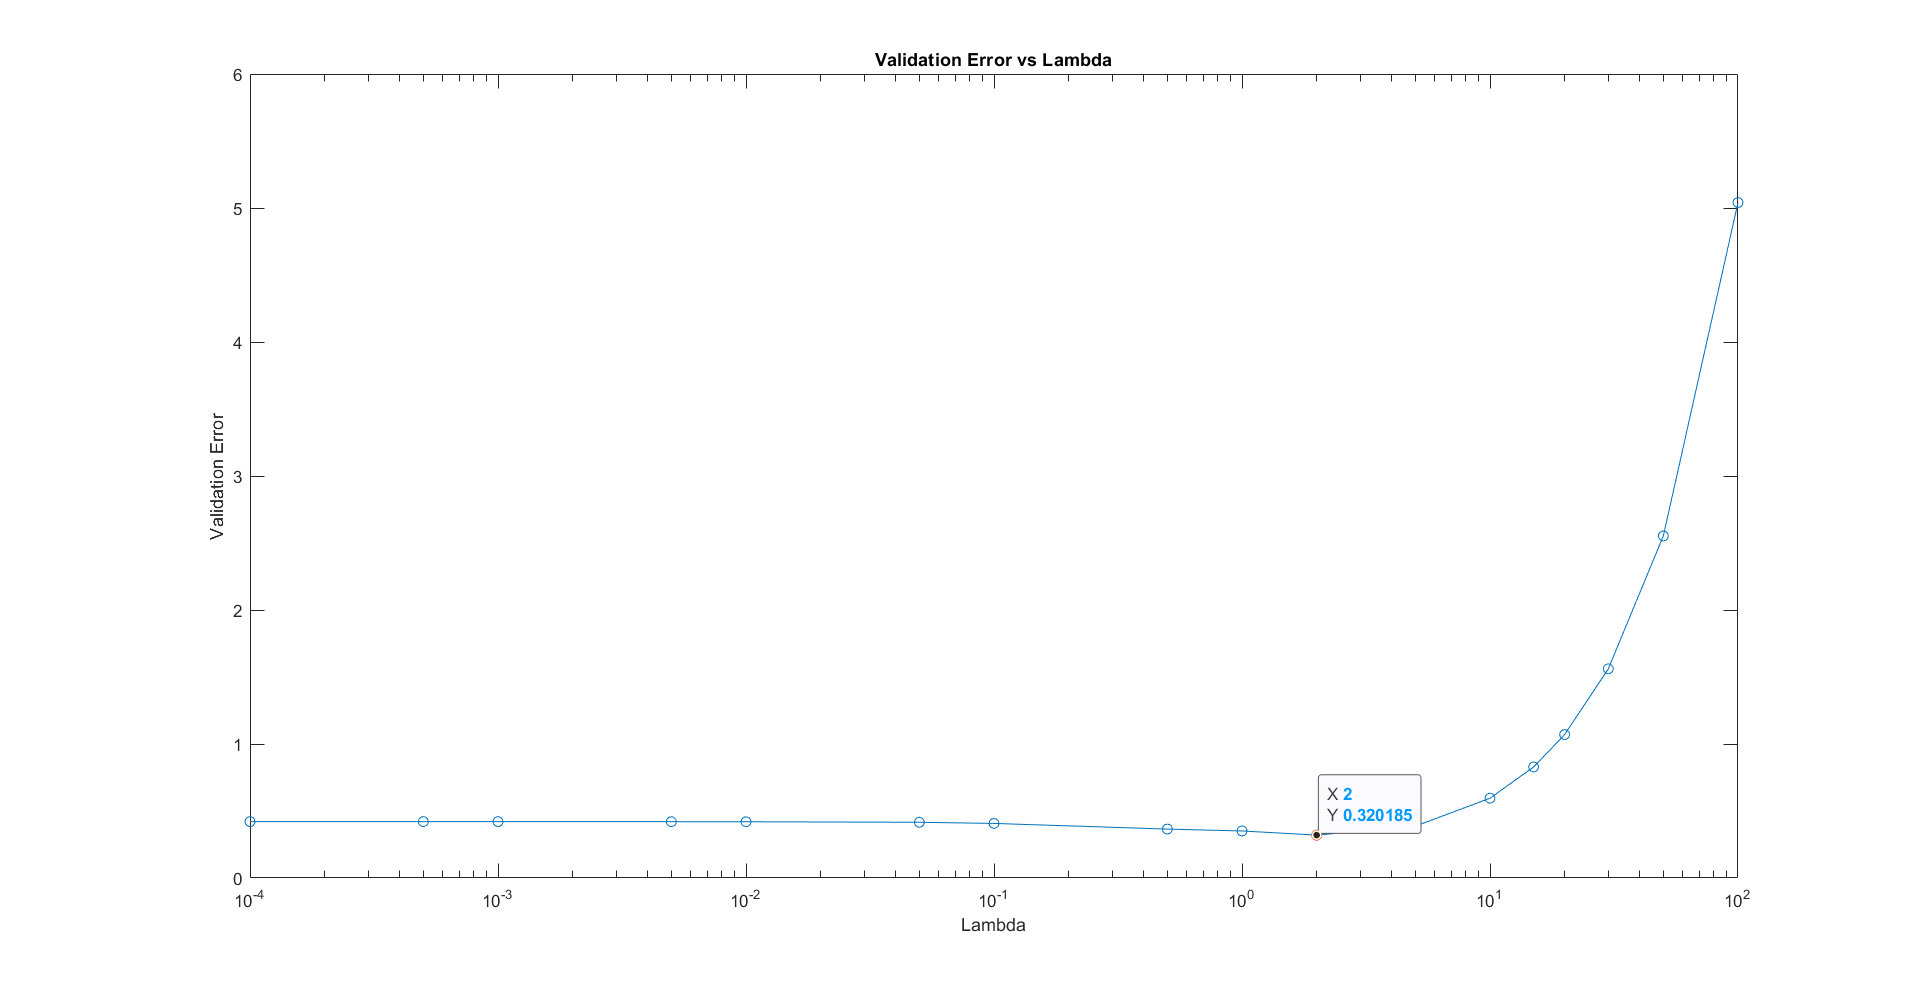
\includegraphics[width=0.9\textwidth]{Images/Q1_VE_vs_lambda.png}
\caption{Plot of $VE$ versus the logarithm of the values in $\Lambda$}
\label{fig:Q1_VE_vs_lambda_1}
\end{figure}

From this plot we can easily see that the validation error is high for higher values of lambda. However, for the values of lambda lower than $5$, the validation error is very low with very little variation. Also, the minimum validation error is obtained for $\lambda = 2$ as highlighted in the figure. Hence, the optimal value of $\lambda$ is $2$.

\begin{figure}[H]
\centering
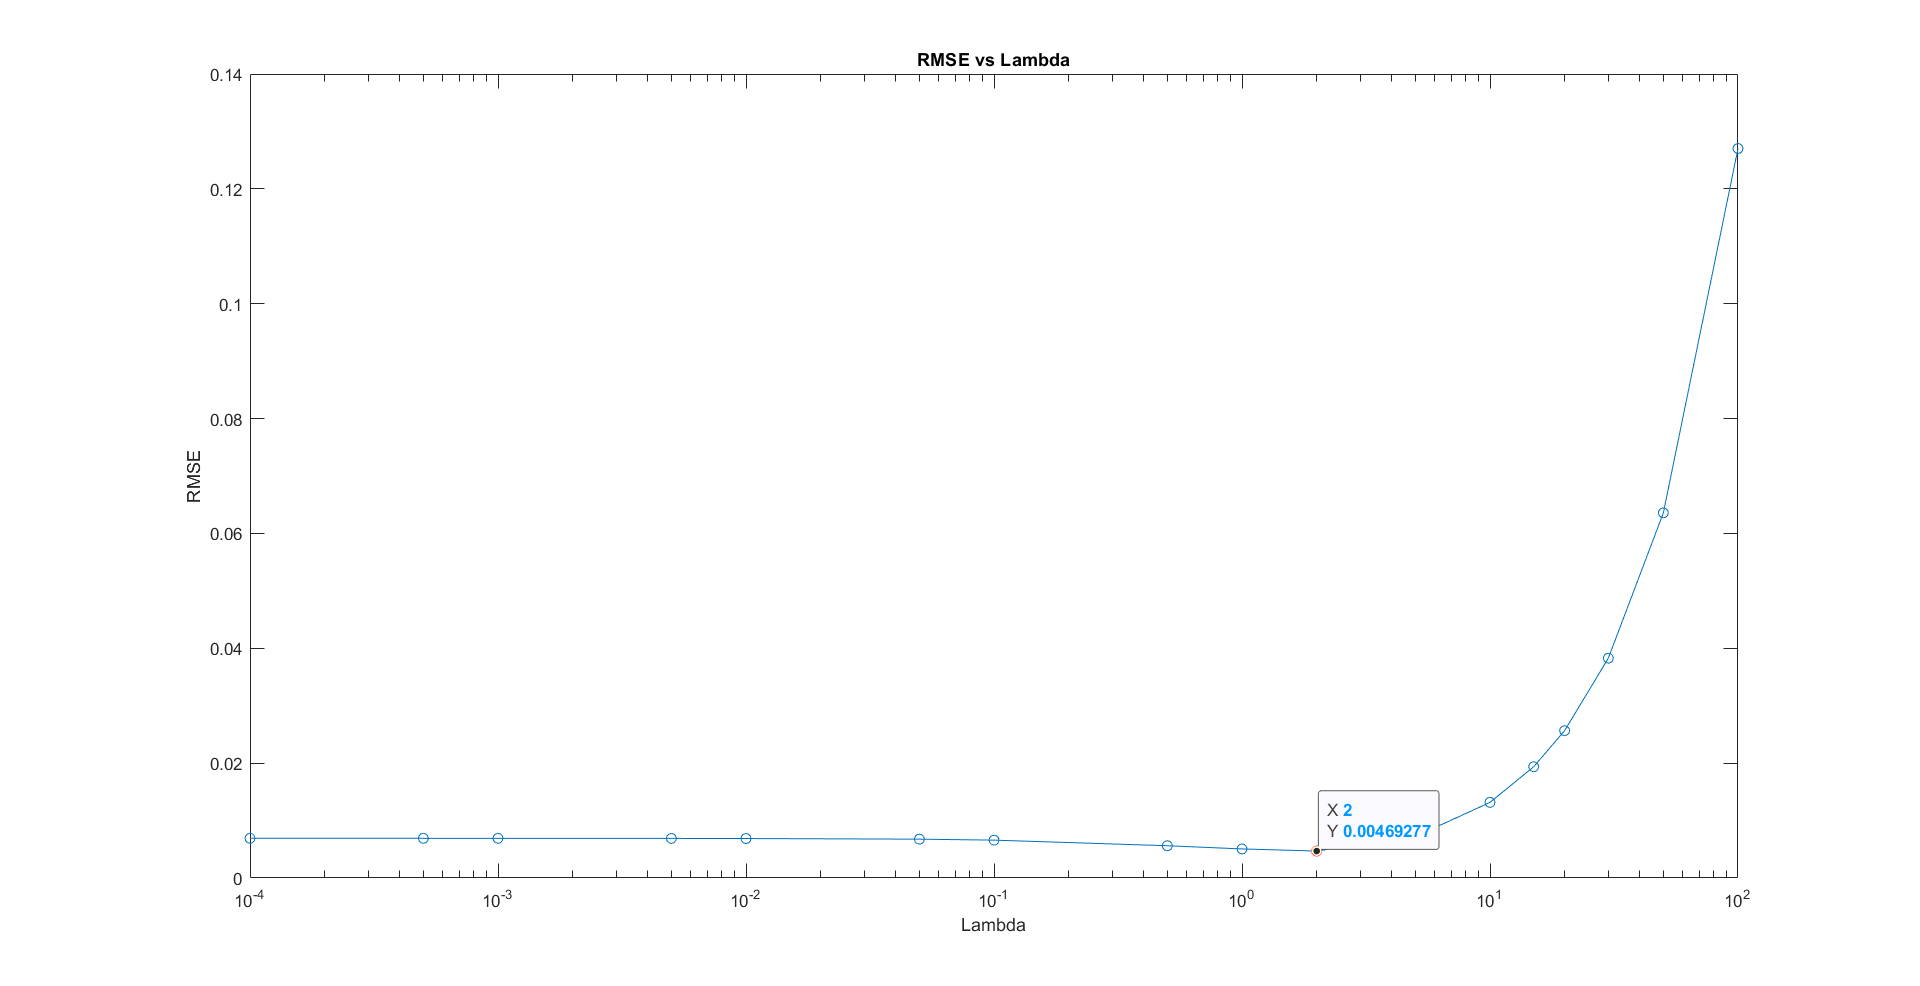
\includegraphics[width=0.9\textwidth]{Images/Q1_RMSE_vs_lambda.png}
\caption{Plot of $RMSE$ versus the logarithm of the values in $\Lambda$}
\label{fig:Q1_RMSE_vs_lambda_1}
\end{figure}
Clearly, the trend of the RMSE vs lambda plot is similar to that of the VE vs lambda plot. Similarly, the RMSE is very low for the values of $\lambda$ greater than $5$ and the optimal value of $\lambda$ is $2$.\\
\textbf{Hence, the value of lambda that we obtain from both the methods is the same.} \\

\item What would happen if $V$ and $R$ were not disjoint but coincident sets? \\
\textbf{Answer:} If $V$ and $R$ are coincident sets, then we are actually attempting to find the value of lambda that minimizes the error on the reconstruction set itself. Clearly, that value of $\lambda$ should be zero as by adding a positive term to $ \| \boldsymbol{y}-\boldsymbol{\Phi x}\|^2 $, we are effectively increasing the value of the objective function $J(\boldsymbol{x})$. Hence, the optimal value of $\lambda$ that is obtained will be close to zero when $V$ and $R$ are coincident sets. This is the reason we need a disjoint validation set (for determining the optimal lambda) which verifies the ability of the algorithm to reconstruct using unseen data.



\item The validation error is actually a proxy for actual mean squared error. Note that you can never determine the mean squared error since the ground truth $\boldsymbol{x}$ is unknown in an actual application. Which theorem/lemma from the paper \url{https://ieeexplore.ieee.org/document/6854225} (On the theoretical analysis of cross-validation in compressed sensing) refers to this proxying ability? Explain how.  \\
\textbf{Answer:} In the given paper, the \textbf{Theorem 1} and \textbf{Theorem 2} prove the proxying ability of the validation error. \\

Theorem 1 (Recovery error estimation) provides bounds on the recovery error $\epsilon_x$ (i.e. the actual MSE) in terms of the Cross validation (CV) residual $\epsilon_{CV}$ (i.e. the validation error). Moreover, it has been shown that this bound becomes tighter as the number of CV measurements ($m_{CV}$) increases. Hence if we have sufficiently large number of CV measurements, and we obtain the hyperparameters that reduce the validation error, then those hyperparameters also reduce the actual mean squared error. \\

Theorem 2 (Recovery error comparison) states that if $\hat{x^p}$ and $\hat{x^q}$ are two recovered signals such that the actual MSE $\epsilon_x^p \geq \epsilon_x^q$, then the validation errors also follow $ \epsilon_{CV}^p \geq \epsilon_{CV}^q$ with probability that increases as the number of CV measurements increases. Hence, if we have sufficiently large number of CV measurements, and we obtain the hyperparameters that reduce the validation error, then those hyperparameters also reduce the actual mean squared error. \\

Hence, we can indeed use the validation error as a proxy for the actual mean squared error given that we have sufficiently large number of CV measurements.

\item In your previous assignment, there was a theorem from the book by Tibshirani and others which gave you a certain value of $\lambda$. What is the advantage of this cross-validation method compared to the choice of $\lambda$ using that theorem? Explain.
\end{enumerate}\\
\textbf{Answer:} The theorem from the book by Tibshirani and others gives us a bound on the value of $\lambda$ as 
\begin{gather*}
    \lambda_m > 2\frac{\phi^T \eta}{m}
\end{gather*}
where $\phi$ is a $m \times n$ matrix. Furthermore, for Gaussian noise the authors showed that the appropriate choice with high probability is 
\begin{gather*}
    \lambda_m = 2\sigma\sqrt{\frac{\tau log(n)}{m}}
\end{gather*}
for some $\tau > 2$ and $\sigma$ is the standard deviation of the noise.\\
However, this choice is only valid if sensing matrix $\phi$ satisfies the restricted eigenvalue condition with parameter $\tau$ for some cone C. The cross validation method does not require such assumption on sensing matrix $\phi$. \\
Moreover, checking the eigenvalue condition is computationally expensive compared to performing cross validation over a set of possible $\lambda$ values. Hence, the cross validation method is more efficient.



\end{itemize}
\end{document}
